
\section{Fast Multipole Methods}\label{chpt:fmm:sec:analytical}

\subsection{Intuition}

As in the original presentation, we use the case of evaluating electrostatic potentials to motivate the \acrshort{fmm}. Consider the electric field, $\mathbf{E}$ due to a static charge distribution $q(\Ybf)$ which is supported over some finite domain $\Ybf \in \Omega \subset \Rd$. It can be defined in terms of a scalar potential $\phi$.

\begin{equation*}
\mathbf{E} = -\nabla \phi
\end{equation*}

which itself can be seen to satisfy Poisson's equation,

\begin{equation*}
    \begin{cases}
        - \Delta \phi(\Xbf) = q(\Xbf), \> \> \text{  for } x\in \Rd \\
        \underset{|x| \rightarrow \infty}{\lim } u(\Xbf) = 0
    \end{cases}
\end{equation*}


where $d=2,3$ in problems of interest.

We can write the evaluation of the potential at a point $\Xbf$ as a convolution of the source with the fundamental solution of the Poisson equation,

such that,

\begin{equation}
\phi(\Xbf) = \int_{\Rd} K(\Xbf-\Ybf)q(\Ybf) d\Ybf, \> \> \Xbf \in \Rd
\end{equation}\label{eq:chpt:fmm:laplace_potential_integral}

Under an appropriate discretisation, where care is taken to appropriately handle the singularity in the Laplace kernel (\ref{eq:chpt:introduction:sec:motivation:laplace_kernel}), we see that this integral corresponds to a matrix vector multiplication, where the matrix is \textit{dense}, i.e. it consists only of non-zero entries.

As we are principally concerned with the simpler problem of evaluating the potential due to a discrete charge distribution, with $N$ charges we can replace $q(\Ybf)$ with $\{ q(\Ybf_j) \}_{j=1}^N$ associated with \textit{source particles} $\{\Ybf_j\}_{j=1}^N \in \Rd$, the integral for potential evaluated at $M$ \textit{target particles}, $\{\Xbf_i \}_{i=1}^M \in \Rd$ becomes a discrete sum,

\begin{equation}
    \phi(\Xbf_i) = \sum_{j=1}^N K(\Xbf_i-\Ybf_j)q(\Ybf_j), \> \> i = 1,...,M
    \label{eq:chpt:fmm:laplace_potential_sum}
\end{equation}

where we can handle the singularity by setting,

\begin{equation}
    K(\Xbf_i - \Ybf_j) = \begin{cases}
        0, \> \> \Xbf_i = \Ybf_j \\
        K(\Xbf_i - \Ybf_j), \text{  otherwise}
    \end{cases}
\end{equation}


We see that the sum (\ref{eq:chpt:fmm:laplace_potential_sum}) corresponds to a dense matrix vector multiplication,

\begin{equation}
    \phi = K q
\end{equation}


\begin{figure}
    \centering
    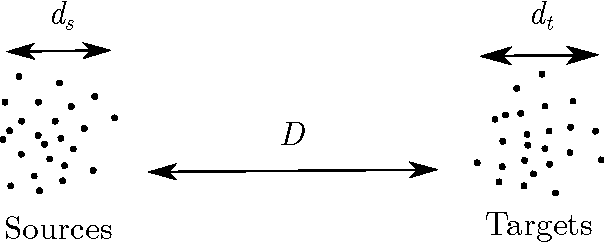
\includegraphics[width=0.5\textwidth]{introduction/degenerate_kernel.pdf}
    \caption{A set of source and target particle cluster, where the width of each cluster is significantly less than the distance separating them, $d_s, d_t \ll D$.}
    \label{fig:chpt:fmm:degenerate_kernel}
\end{figure}

Naively computed this requires $\bigO{MN}$ operations, where in general the source and target particles may correspond to the same set. The \acrshort{fmm} relies on a \textit{degenerate} approximation of the interaction kernel when subsets, or \textit{clusters}, of source and target particles are sufficiently separated as sketched in Figure \ref{fig:chpt:fmm:degenerate_kernel}. Following the discussion in \cite{kailasa2024m2ltranslationoperatorskernel} the sum (\ref{eq:chpt:fmm:laplace_potential_sum}) can be written as,

\begin{equation}
    \phi(\Xbf_i) \approx \sum_{p=1}^P \sum_{j=1}^N A_p(\Xbf_i) B_p(\Ybf_j)q(\Ybf_j), \> \> i = 1,...,M
    \label{eq:chpt:introduction:sec:motivation:degenerate_kernel}
\end{equation}

where we call $P$ the expansion order, taken such that $P \ll N$, $P \ll M$. The functions $A_p$ and $B_p$ are defined by the approximation scheme used by a particular approach for the \acrshort{fmm}, in the original presentation the calculation,

\begin{equation}
    \hat{q}_p = \sum_{j=1}^N B_p(\Ybf_j)q(\Ybf_j)
\end{equation}

Corresponded to the coefficients of an order $P$ multipole expansion due to the source charges. Following which the potential is approximated by,

\begin{equation}
    \phi(\Xbf_i) \approx \sum_{p=1}^P A_p(\Xbf_i)\hat{q}_p, \> \> i = 1,...,M
\end{equation}

at the target particles. The approximation of the potential with this scheme can be seen to require $\bigO{P(M+N)}$ operations. The accuracy of this approximation scheme, and the error bounds provided by the \acrshort{fmm}, depends on the distance between the source and target clusters remaining large relative to their width. This condition is often referred to as an \textit{admissibility condition} in the \acrshort{fmm} literature. \acrshort{fmm}s therefore split the sum (\ref{eq:chpt:fmm:laplace_potential_sum}) into \textit{near} and \textit{far} components when considering arbitrary clusters of source and target particles,

\begin{equation}
    \phi(\Xbf_i) = \sum_{\Ybf_j \in \text{Near}(\Xbf_i)} K(\Xbf_i, \Ybf_j) q(\Ybf_j) +  \sum_{\Ybf_j \in \text{Far}(\Xbf_i)} K(\Xbf_i, \Ybf_j) q(\Ybf_j), \> \> i=1,..,M
\end{equation}

In cases where a source and target cluster can be considered \textit{admissable}, i.e. the source cluster is considered in the \textit{far field} of the target cluster such that each $\Ybf_j \in \text{Far}(\Xbf_j)$, we apply the approximation (\ref{eq:chpt:introduction:sec:motivation:degenerate_kernel}). However, when a source and target cluster are \textit{inadmissable}, such that the source cluster is considered in the \textit{near field} of a target cluster such that each $\Ybf_j \in \text{Near}(\Xbf_j)$ we are left to evaluate the sum directly via (\ref{eq:chpt:fmm:laplace_potential_sum}).

In order to achieve its $\bigO{N}$ complexity the \acrshort{fmm} is structured to reduce to a minimum the number of sums evaluated between inadmissable clusters.


\subsection{Algorithm Zoo}

- Chief variants, analytical, semi-analytical, algebraic, where do each of the cited methods apply, what are their shortcomings and advantages, especially in terms of performance.

- Generally considered that low-order analytical and high-order algebraic approaches, for performance however this is not actually known.





\subsubsection{Non-Adaptive Case}

- How are analytical expansions defined, 2D Laplace example, note and references on 3D laplace example.
    - private note on how these derivations are found.

- Note on admissibility, how it defines a broad class of FMM matrices, table of related matrix types with different rank structure and admissability criterion

This is achieved with a hierarchical discretisation of the problem domain, often a \textit{quadtree} in two dimensions and correspondingly an \textit{octree} in three dimensions.

- trees define admissability from geometry for FMM, note on alternative approaches such as ORB.

These data structures are generated by creating a bounding box that covers the source and target particles, which without loss of generality may correspond to the same set. This box is then recursively sub-divided into \textit{child boxes} of equal size.


- Define interaction lists.

- Define all operators.

- Give an algorithm sketch.

- Give complexity sketch.

\subsubsection{Adaptive Case}

- Types of adaptivity available (weak, strong) requirements on interaction lists.

- Define new interaction lists, and new operators

- Give complexity sketch.
